\documentclass[border=4pt]{standalone}
\usepackage{amsmath,amssymb,amsfonts}
\usepackage{xcolor,colortbl,array,booktabs,multirow}
\usepackage{tikz}
\usepackage{pgfplots}
\pgfplotsset{compat=1.16}
\usetikzlibrary{arrows, automata, backgrounds, calendar, chains, decorations,
    matrix, mindmap, patterns, petri, positioning, shadows, shapes.geometric,
    trees, shapes, decorations.pathreplacing, calc, tikzmark, arrows.meta,
    intersections, fit, graphs, quotes, angles, decorations.markings}
\newcommand{\st}{\text{ s.t. }}
\newcommand{\x}{\mathbf{x}}
\renewcommand{\b}{\mathbf{b}}
\renewcommand{\c}{\mathbf{c}}
\newcommand{\A}{\mathbf{A}}
\newcommand{\y}{\mathbf{y}}
\newcommand{\z}{\mathbf{z}}
\newcommand{\R}{\mathbb{R}}
\newcommand{\RR}{\mathbb{R}}
\newcommand{\Z}{\mathbb{Z}}
\newcommand{\ZZ}{\mathbb{Z}}
\newcommand{\npcomplete}{NP-complete}
\providecommand{\true}{\text{TRUE}}
\providecommand{\false}{\text{FALSE}}
\tikzset{vertex/.style={circle,fill=black!25,minimum size=20pt,inner sep=0pt},
    edge/.style={draw,thick,-},weight/.style={font=\small},
    selected vertex/.style={vertex, fill=red!24},
    selected edge/.style={draw,line width=2pt,-,red!50},
    ignored edge/.style={draw,line width=2pt,-,black!20}}
\newcommand{\vect}{\vec}
\providecommand{\ds}{\displaystyle}
\providecommand{\longvect}{\overrightarrow}
\usepackage[normalem]{ulem}
\definecolor{ocre}{RGB}{243,102,25}
\providecommand{\leftB}{\left[}
\providecommand{\rightB}{\right]}
\tikzset{directed/.style={postaction={decorate,decoration={markings,mark=at position .65 with {\arrow{>}}}}},
    directed1/.style={postaction={decorate,decoration={markings,mark=at position .65 with {\arrow{>}}}}}}
\begin{document}
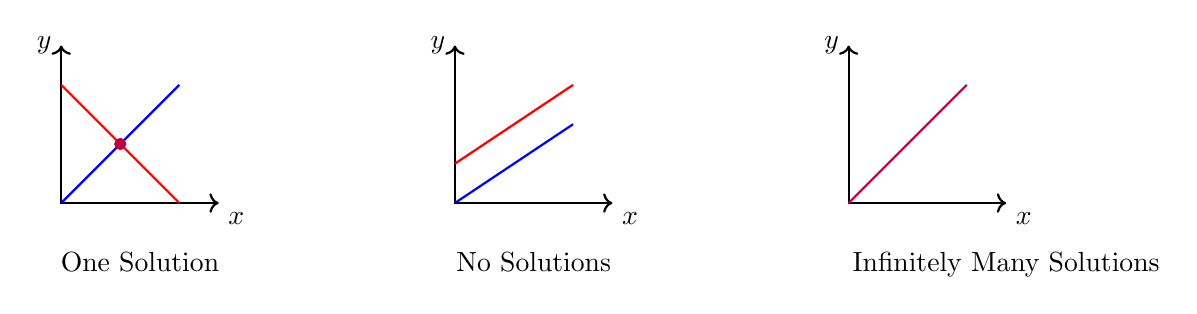
\begin{tikzpicture}
\draw[thick, <->](0,2)--(0,0)--(2,0);
\draw[thick, red](0,1.5)--(1.5,0);
\draw[thick, blue](0,0)--(1.5,1.5);
\draw[fill, purple](0.75,0.75) circle [radius=2pt];
\node[below right] at (2,0){$x$};
\node[left] at (0,2){$y$};
\node[below] at (1,-0.5){One Solution};

\draw[thick, <->](5,2)--(5,0)--(7,0);
\draw[thick, red](5,0.5)--(6.5, 1.5);
\draw[thick, blue](5,0)--(6.5,1);
\node[below right] at (7,0){$x$};
\node[left] at (5,2){$y$};
\node[below] at (6,-0.5){No Solutions};

\draw[thick, <->](10,2)--(10,0)--(12,0);
\draw[thick, purple](10,0)--(11.5, 1.5);
\node[below right] at (12,0){$x$};
\node[left] at (10,2){$y$};
\node[below] at (12,-0.5){Infinitely Many Solutions};
\end{tikzpicture}
\end{document}
